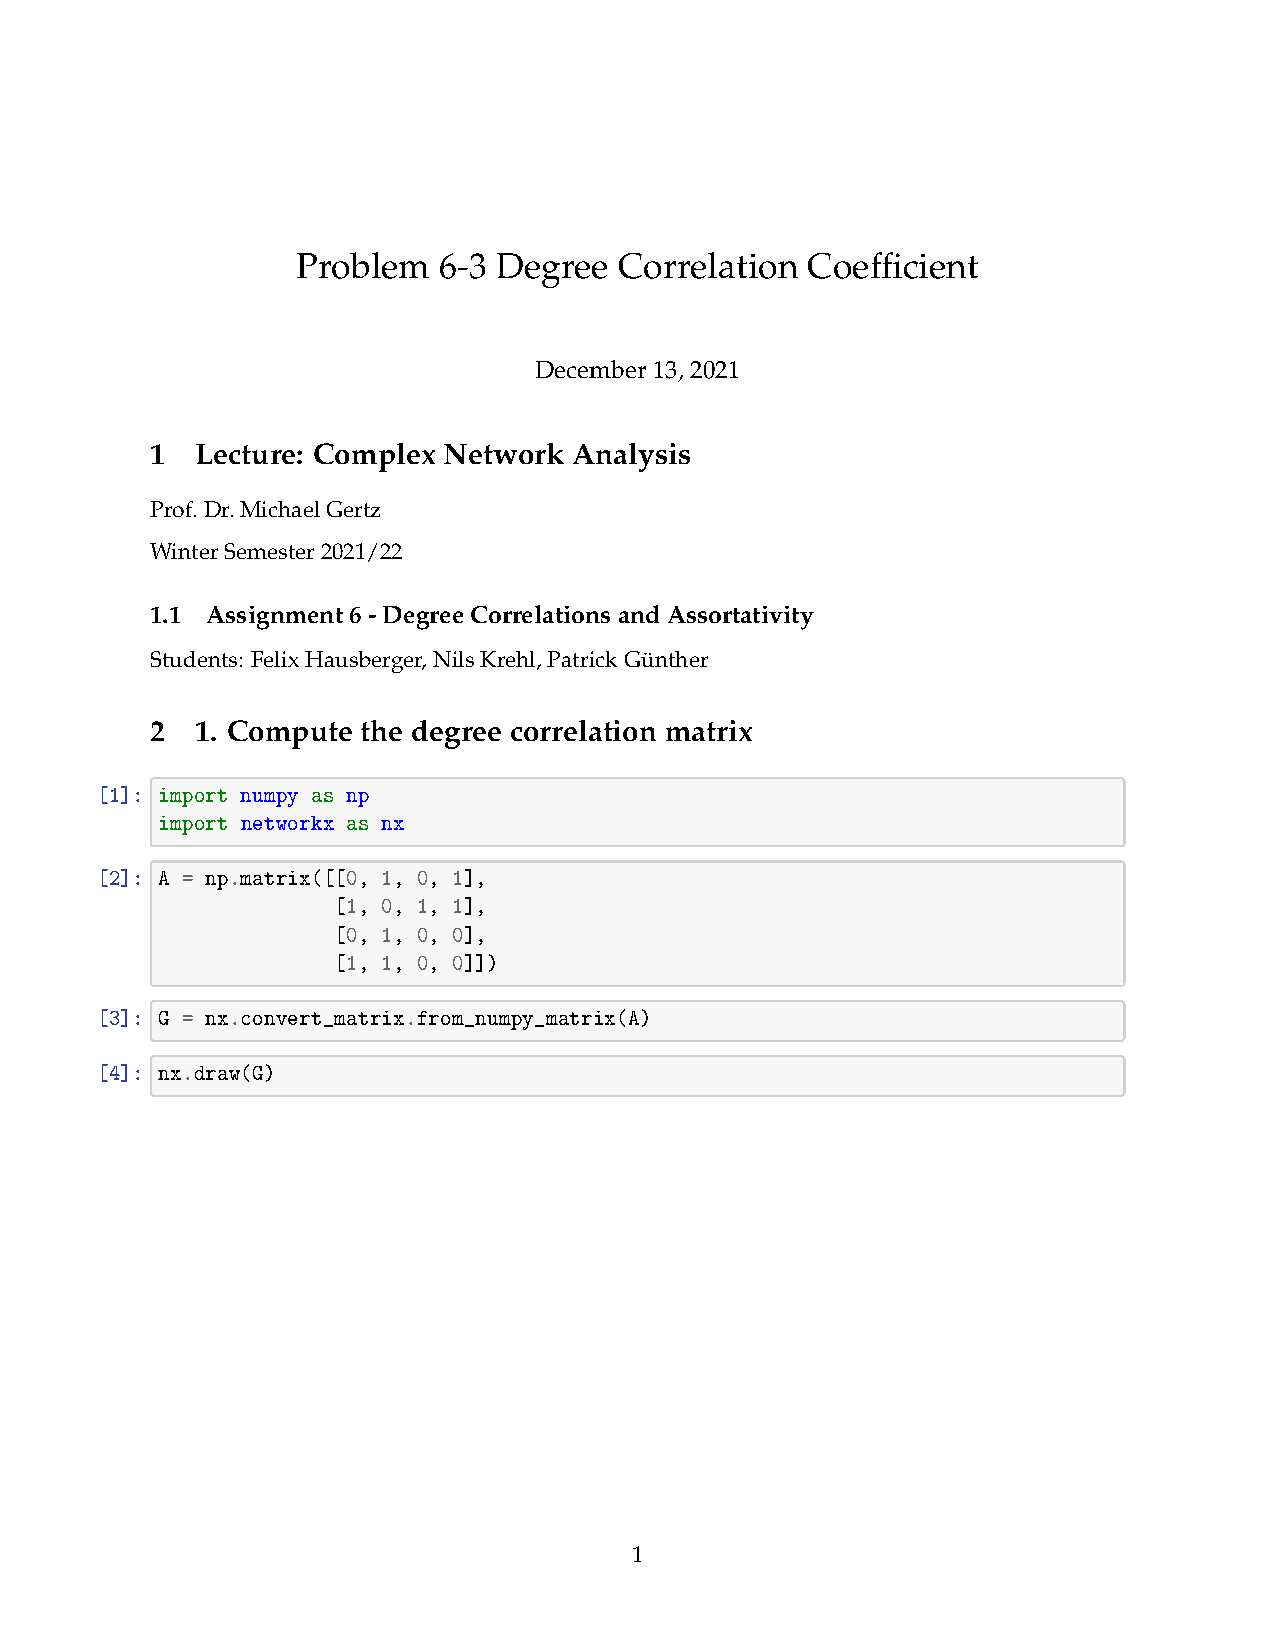
\includepdf[pages=-]{pdfs/problem_3.pdf}

\begin{enumerate}
	\item Compute the degree correlation matrix.
	
	We computed the degree correlation matrix using networkx using inbuild functions (since it is repetitive).  The manual process would be to calculate for each cell of the matrix the fraction of edges which connect nodes with the correct degree of $i$ and $j$.  For example,  in the graph only one edge connects nodes which have the degree $1$ and $3$ with each other.  There are a total of $4$ edges in the graph.  Normalized, so that $E$ sums up to $1$ (and since $e_{ij}$ as well as $e_{ji}$ are always taken into account) the cells $e_{1,3}$ and $e_{3,1}$ have a value of $0.125$. The same process goes for the remaining cells. The degree correlation matrix is shown in Table \ref{tab:deg_corr_mat}.
	
	\begin{table}[h]
	\centering
	\begin{tabular}{lllll}
		\hline
		\textbf{}  & \textbf{0} & \textbf{1} & \textbf{2} & \textbf{3} \\ \hline
		\textbf{0} & 0          & 0          & 0          & 0          \\ \hline
		\textbf{1} & 0          & 0          & 0          & 0.125      \\ \hline
		\textbf{2} & 0          & 0          & 0.25       & 0.25       \\ \hline
		\textbf{3} & 0          & 0.125      & 0.25       & 0          \\ \hline
	\end{tabular}
	\caption{Degree Correlation Matrix}
	\label{tab:deg_corr_mat}
	\end{table}
	
	\item Compute the probabilities $q_k$.
	
	We used formula 7.3 from the lecture slides.  The results are shown in Table \ref{tab:qk}
	
	\begin{table}[h]
	\centering
	\begin{tabular}{|l|l|}
		\hline
		\textbf{$k$} & \textbf{$q_k$} \\ \hline
		0          & 0.000         \\ \hline
		1          & 0.125         \\ \hline
		2          & 0.500         \\ \hline
		3          & 0.375         \\ \hline
	\end{tabular}
	\caption{}
	\label{tab:qk}
	\end{table}

  \item Compute the degree correlation coefficient r.
  
  Our solution is $r = -0.714$. We used formula $7.11$ from the lecture slides. 
  
  Since $r < 0$, the network is disassortative.
\end{enumerate}